\section{Giới thiệu}

\begin{frame}{Động lực nghiên cứu}
	\vspace{5pt}
	
	\begin{columns}
	% Left column
	\begin{column}{0.7\textwidth}
		\textbf{Text-base Deep Learning}
		\begin{itemize}
			\item ChatGPT, Alexa, Character.AI,..
			\item Text to speech, text to text,..
		\end{itemize}
		
		\textbf{Text/audio to Realistic Digital Humam}
		
		\begin{itemize}
			\item Video-base (HeyGen, Midjourney,...)
			\item Rendering-base:
			\begin{itemize}
				\item Character model (Gaussian Splatting)
				\item Character animation: (3D keypoints)
			\end{itemize}
		\end{itemize}
		\vspace{5pt}
		\centering
		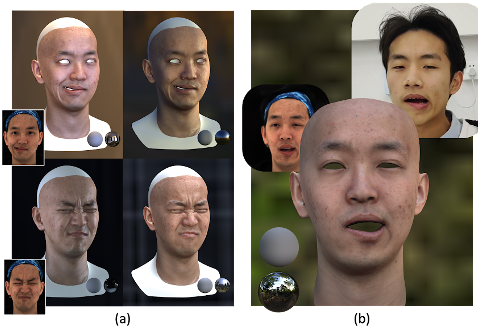
\includegraphics[width=0.8\textwidth]{FacialAsset.png}
	\end{column}
	
	% Right column
	\begin{column}{0.3\textwidth}
		\begin{figure}
				
\includegraphics[width=\textwidth]{UniversalHuman.png}
%				\caption{\small Minh hoạ người kỹ thuật số siêu thật (realistic digital human)}
		\end{figure}
		
		\begin{figure}
			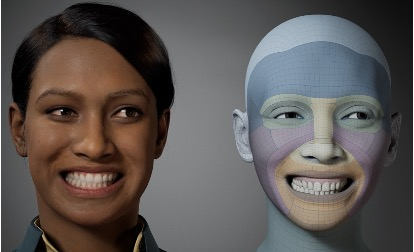
\includegraphics[width=\textwidth]{MetaHuman.jpg}
			\caption{\small Minh hoạ người kỹ thuật số siêu thật (realistic digital human)}
		\end{figure}
	
	\end{column}
	
	\end{columns}
\end{frame}



\begin{frame}{Dữ liệu bài toán}
	
	
	\begin{columns}
		
		\begin{column}{0.7\textwidth}
			
			\textbf{Dữ liệu}
			\begin{itemize}
				\item Dữ liệu chuyển động thu nhận từ cảm biến.
				\item Âm thanh tương ứng với cử chỉ.
			\end{itemize}
			
			\textbf{Kiến trúc khung xương trong file BVH}
			\begin{itemize}
				\item \textbf{HIERARCHY}: Định nghĩa vị trí và thành phần trong khung xương.
				\begin{itemize}
					\item Skeleton: 75 bones : 
%					\mathbf{B} =
					\small{(\texttt{Head}, \texttt{Spine}, \texttt{Hips}, \texttt{LeftArm},\texttt{RightArm}... )} \\
%					Dữ liệu BVH: $\mathbf{b}_{i} = \{r_x, r_y, r_z\}$
				\end{itemize}
				\item \textbf{MOTION}: Chuỗi chuyển động khung xương $60 \text{fps}$
				\begin{figure}[h]
					\centering
					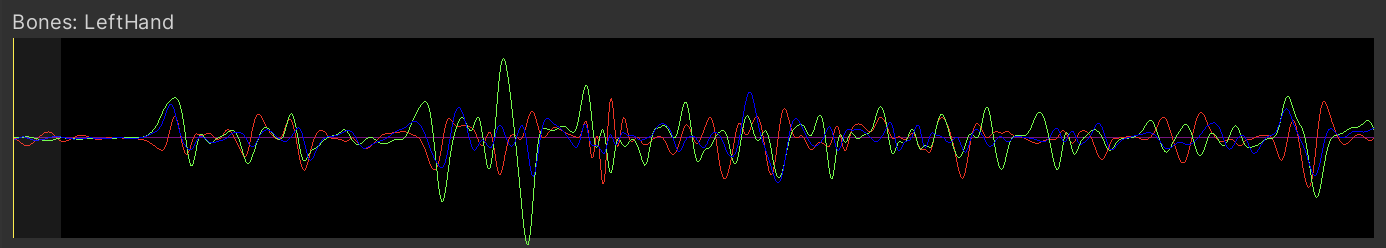
\includegraphics[width=0.9\textwidth]{BoneRotationSeries}
				\end{figure}
				
				
			\end{itemize}
			Dữ liệu sau xử lý: $\mathbf{g} \in \mathbb{R}^{D}$, với $D=1141$ 
			$\mathbf{g} = \Big[ \mathbf{p},  \mathbf{r},
			\mathbf{ p }',  \mathbf{r}',
			\mathbf{p}_{\text{joins}},  \mathbf{r}_{\text{joins}},
			\mathbf{p}'_{\text{joins}},  \mathbf{r}'_{\text{joins}},
			\mathbf{d}_{\text{gaze}}
			\Big]$
%			\textbf{Loại bài toán}: Hồi quy (regression)
%			\begin{itemize}
%				\item Cho trước $N$ khung hình (frame) cử chỉ, dự đoán $M$ khung hình tiếp theo tương ứng với âm thanh $\mathbf{a}$.
%			\end{itemize}
		
		\end{column}
		
			\begin{column}{0.3\textwidth}
				\begin{figure}[h]
					\centering
					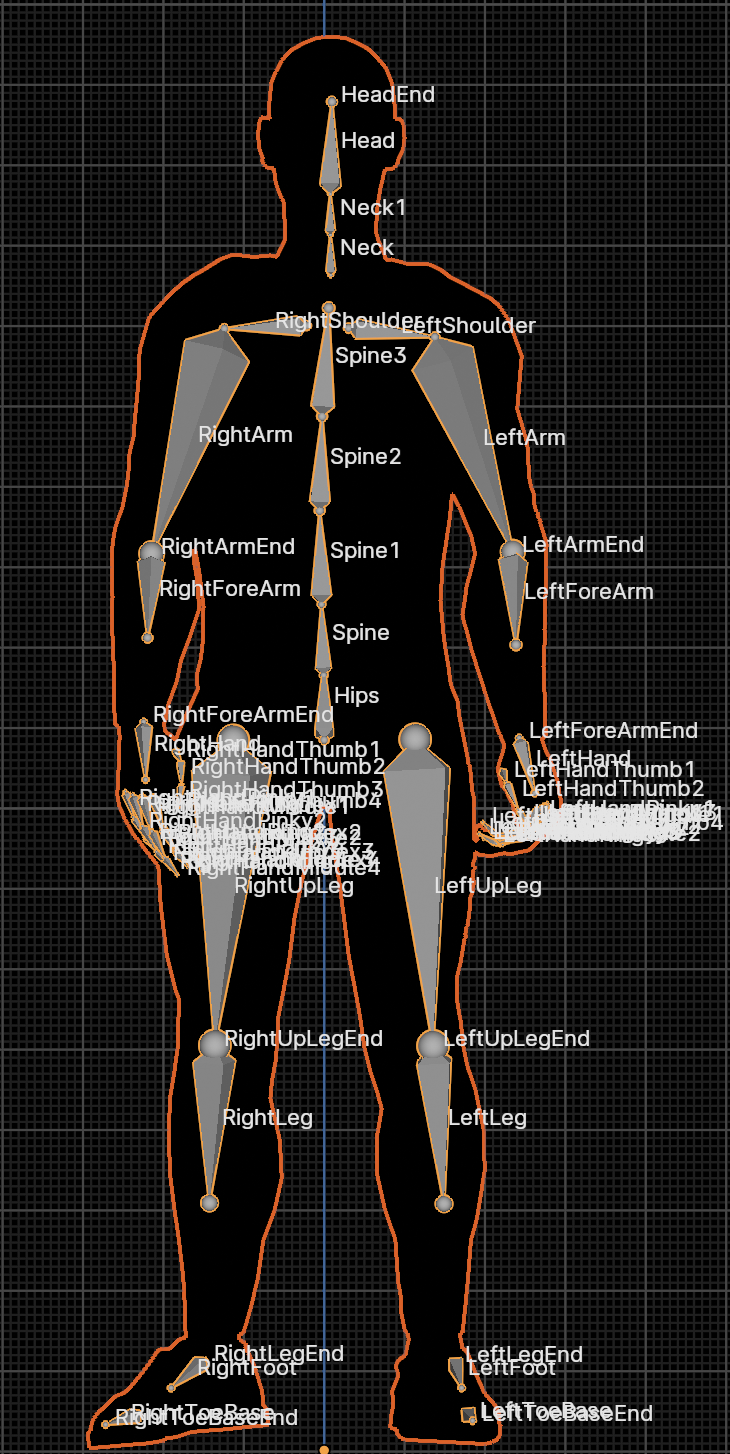
\includegraphics[width=\textwidth]{Skeleton}
				\end{figure}
		\end{column}
		
	\end{columns}
	
\end{frame}

\begin{frame}{Chuyển động của tọa độ}
		\begin{figure}
		\centering
		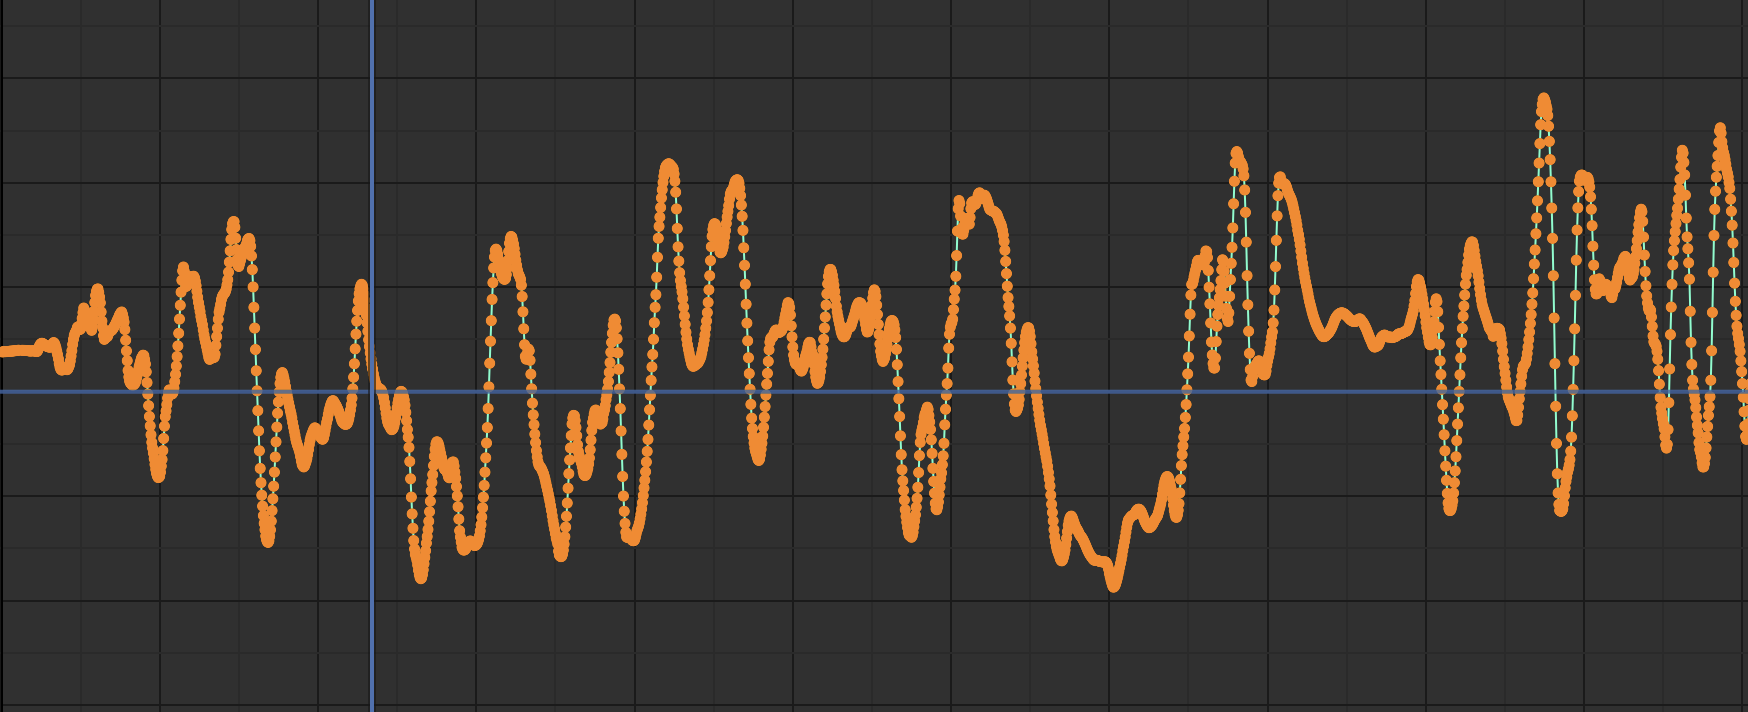
\includegraphics[width=\textwidth, height=40pt]{MotionXYZ.png}
		\caption{Minh hoạ chuyển động của góc quay một Bone trong tọa độ}
	\end{figure}
	\vspace{-15pt}
	\begin{columns}
		\begin{column}{0.78\textwidth}
			$$
			D = 3 + 4 + 3 + 3 + 3 \times 75 + 6 \times 75 + 3 \times 75 + 3 \times 75 + 3
			$$
			\vspace{-20pt}
			\begin{itemize}
				\item $\mathbf{p} \in \mathbb{R}^3$: tọa độ của điểm gốc
				\item $\mathbf{r} \in \mathbb{R}^4$: Góc quay của điểm gốc
				\item $\mathbf{p}'_{\text{root}} \in \mathbb{R}^3$: Vận tốc thay đổi của tọa độ gốc
				\item $\mathbf{r}'_{\text{root}} \in \mathbb{R}^3$: Vận tốc thay đổi của góc quay gốc
				
				\item $\mathbf{p}_{\text{joins}} \in \mathbb{R}^{3 n_{\text{join} }}$: tọa độ của các khung xương
				\item $\mathbf{r}_{\text{joins}} \in \mathbb{R}^{6 n_{\text{join} }}$: Góc quay của các khung xương
				\item $\mathbf{p}'_{\text{joins}} \in \mathbb{R}^{3n_{\text{join} }}$: Vận tốc thay đổi của tọa độ các khung xương
				\item $\mathbf{r}'_{\text{joins}} \in \mathbb{R}^{3n_{\text{join} }}$: Vận tốc thay đổi của góc quay các khung xương
				
				\item $\mathbf{d}_{\text{gaze}} \in \mathbb{R}^3$: Là hướng nhìn
			\end{itemize}
		\end{column}
		
		\begin{column}{0.22\textwidth}
			\vspace{12pt}
			\begin{figure}
				\centering
				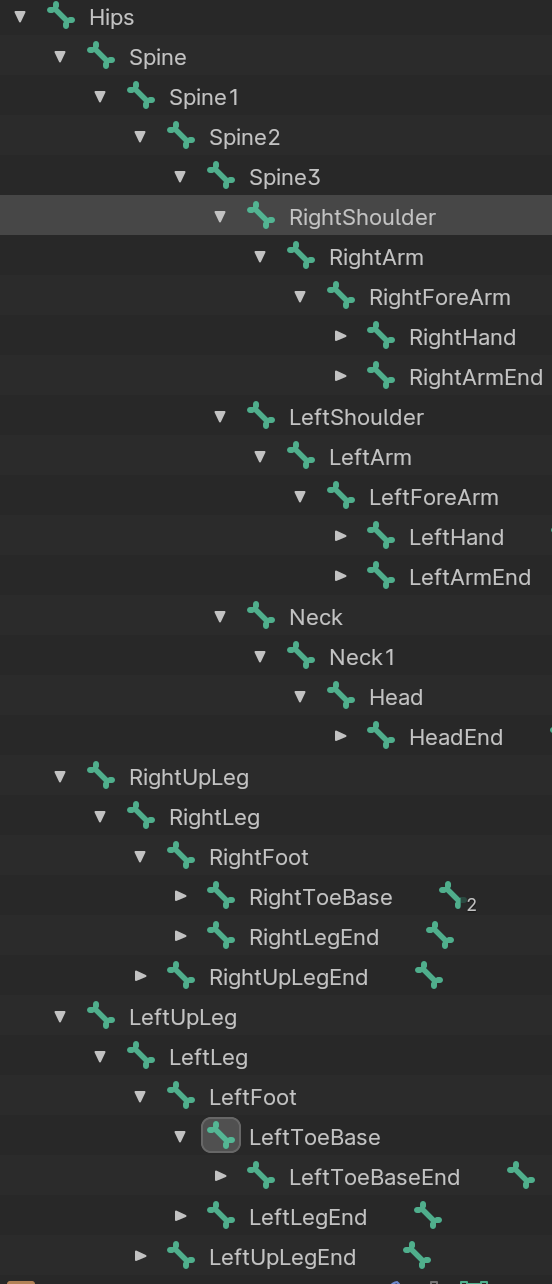
\includegraphics[width=\textwidth]{Bone.png}
			\end{figure}
			
		\end{column}
	\end{columns}
	
\end{frame}

\begin{frame}
%	Mỗi Bone được biểu diễn thành: 
%	$$q = w + xi + yj + zk$$
%	
%	$$i^2 = j^2 = k^2 = ijk = -1$$
	\begin{figure}
		\centering
		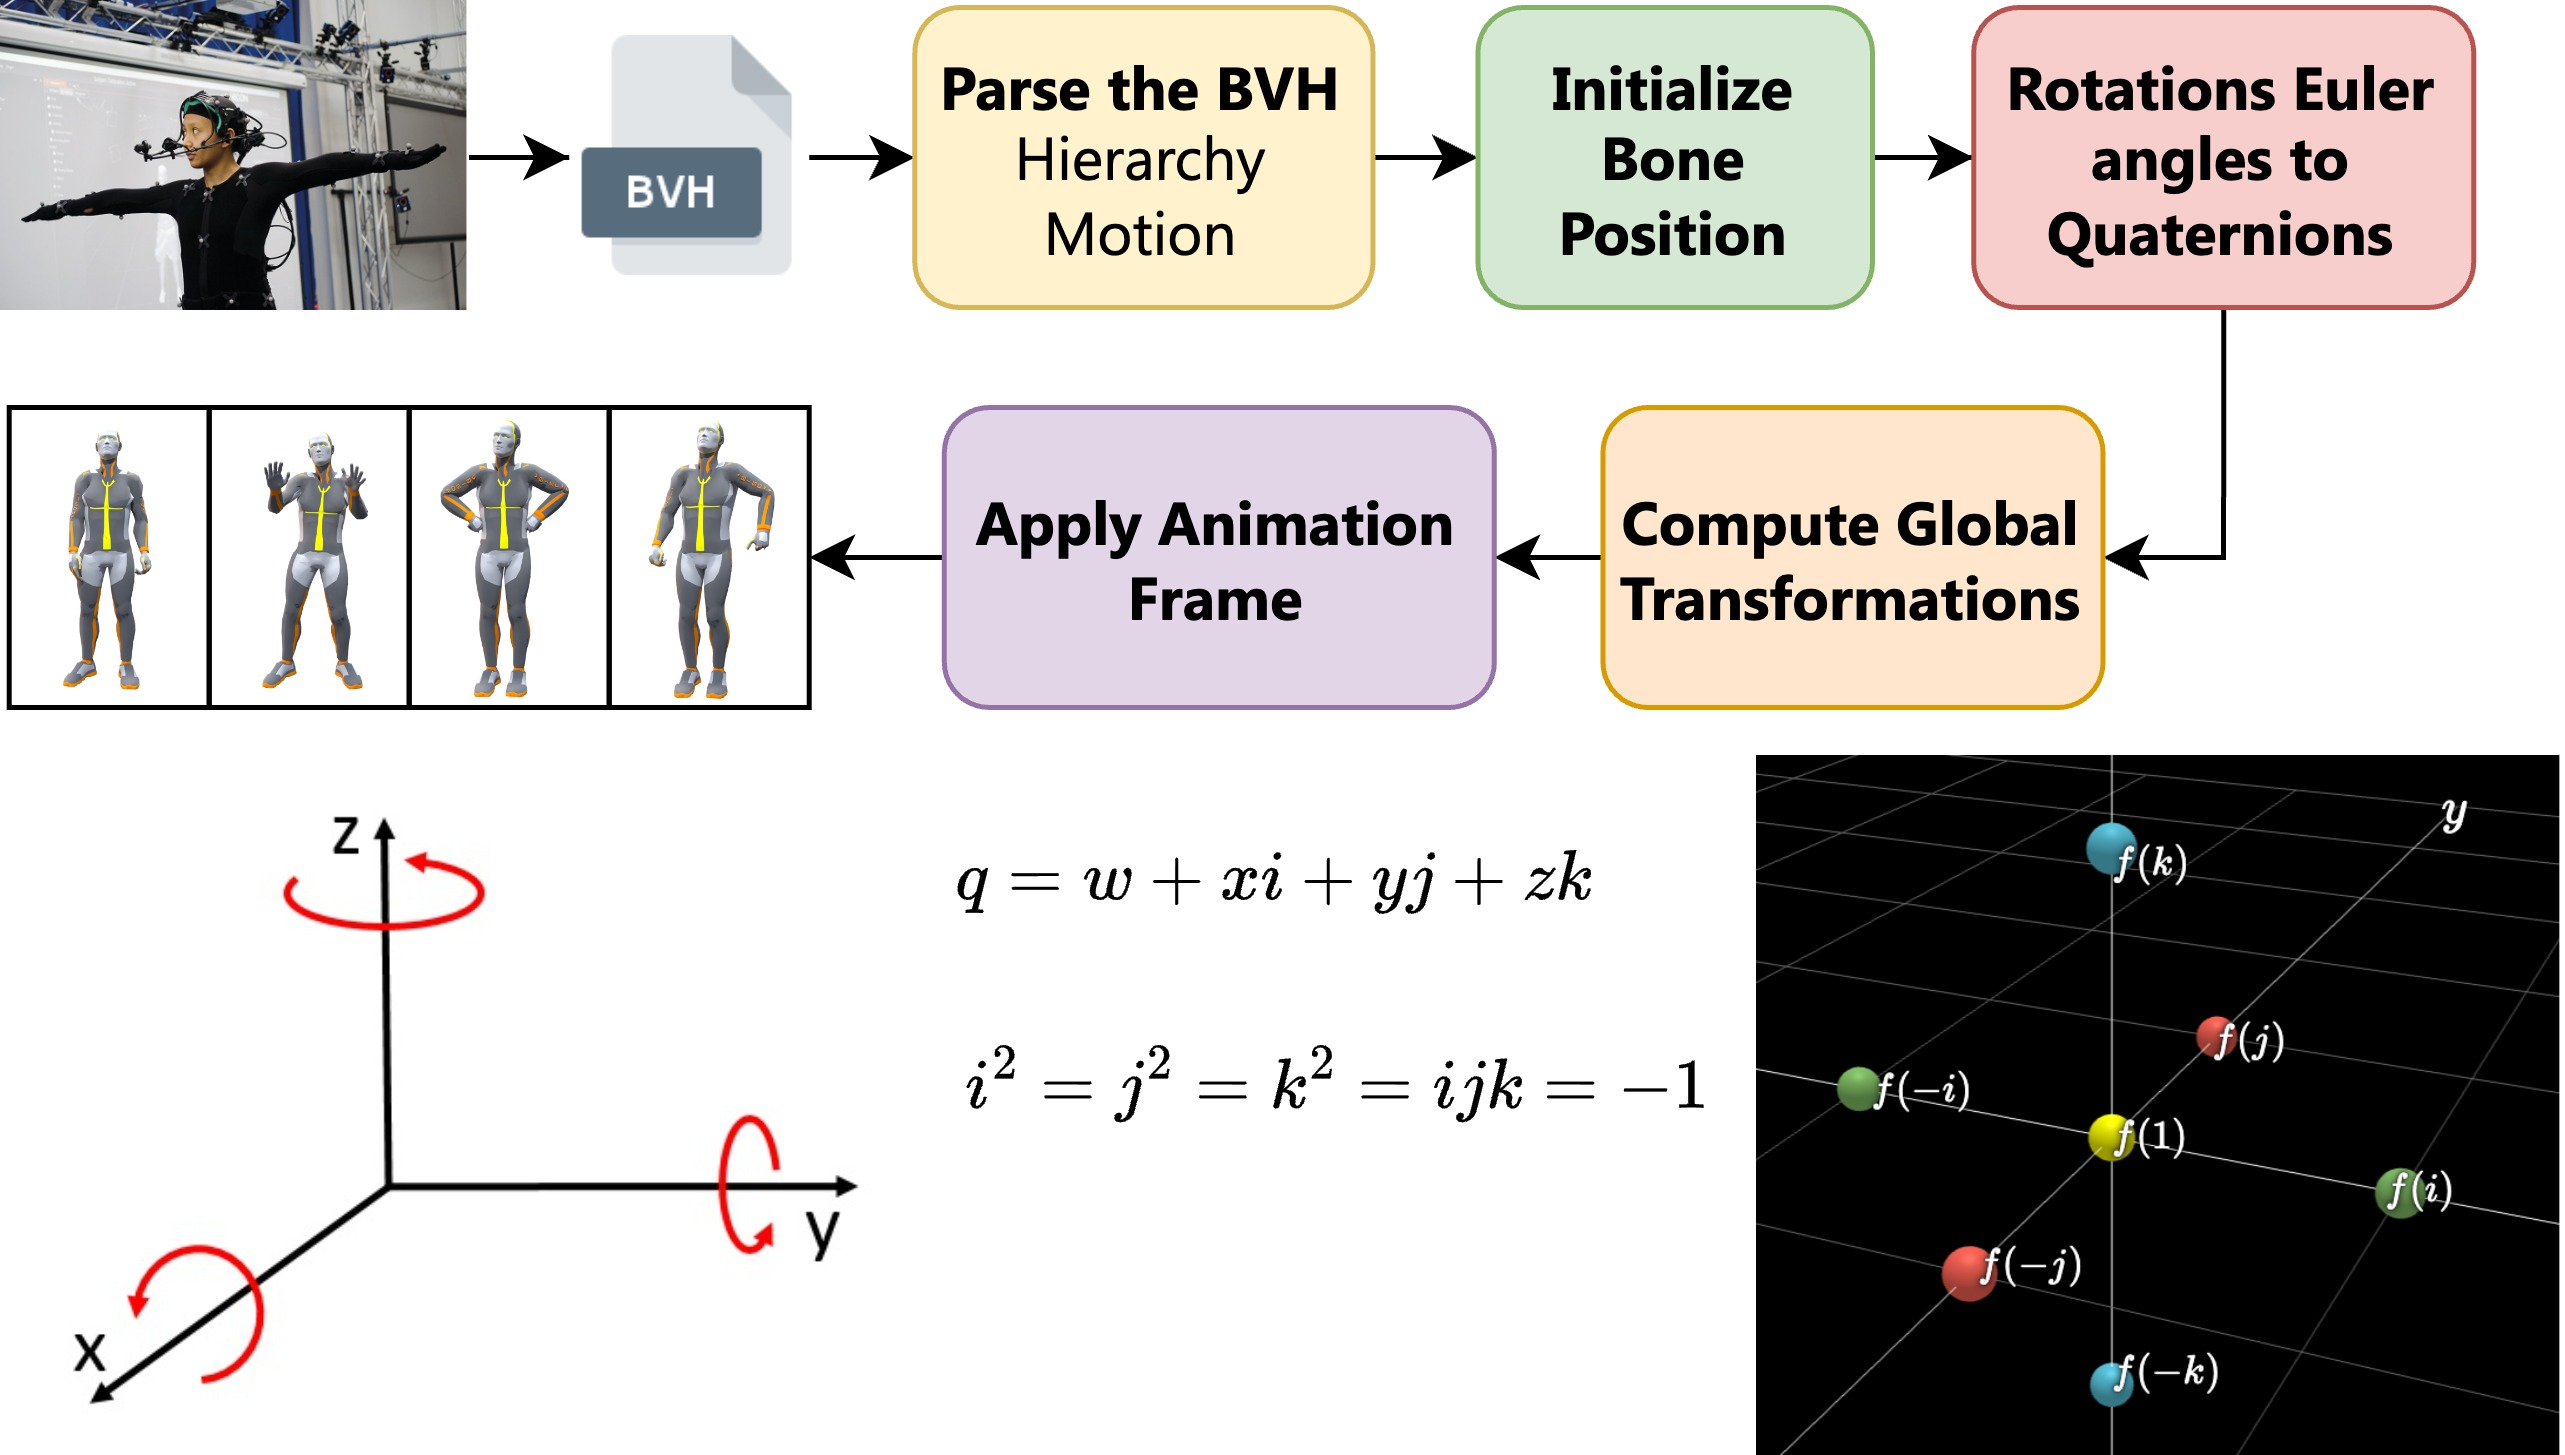
\includegraphics[width=\textwidth]{BVH}
	\end{figure}
\end{frame}


\begin{frame}{Góc quay của một khung xương}
	\small
	\textbf{Hierachy}: bao gồm 75 Bone $\{ \mathbf{t}_i \}^{75} $, có vị trí ban đầu  $\mathbf{t}_{i} = \{t_x, t_y, t_z\}$
	
	\vspace{5pt}
	
	\textbf{Bone} trong dữ liệu BVH bao gồm vị trí $\mathbf{position}_{\operatorname{local}}  \in \mathbb{R}^{3}$ và góc quay $\mathbf{rotation}_{\operatorname{local}} \in \mathbb{R}^{3}$.
%	\begin{figure}
%		\centering
%		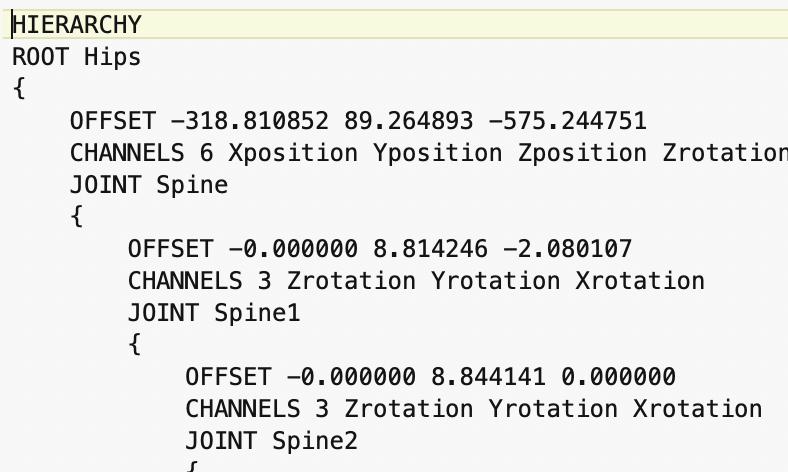
\includegraphics[width=0.25\textwidth]{BVHFile}
%	\end{figure}
	$\mathbf{rotation}_i^{\operatorname{local}} = \{ \alpha ,\beta , \gamma \}$ lần lượt là góc quay quanh các trục $Z$ ,$Y$ , và $X$, góc quay tổng hợp trong không gian Eule là $R = R_Z(\alpha) R_Y(\beta) R_X(\gamma)$:
	\begin{equation}
		\mathbf{position}_{\text{global}} = R \cdot \mathbf{position}_{\text{local}} + \mathbf{t}
	\end{equation}
	Chuyển góc quay từng Bone dạng Euler ZYX sang dạng Quaternion, mỗi Bone biểu diễn bằng $q = (q_w, q_x, q_y, q_z)$
	%	Mỗi Bone được biểu diễn thành: 
	%	$$q = w + xi + yj + zk$$
	%	c
	%	$$i^2 = j^2 = k^2 = ijk = -1$$
	\begin{columns}
		\begin{column}{0.5\textwidth}
			\begin{itemize}
				\item $c_{\alpha} = \cos\left(\frac{\alpha}{2}\right), \quad s_{\alpha} = \sin\left(\frac{\alpha}{2}\right)$
				\item $c_{\beta} = \cos\left(\frac{\beta}{2}\right), \quad s_{\beta} = \sin\left(\frac{\beta}{2}\right)$
				\item $c_{\gamma} = \cos\left(\frac{\gamma}{2}\right), \quad s_{\gamma} = \sin\left(\frac{\gamma}{2}\right)$
			\end{itemize}
		\end{column}
		\begin{column}{0.5\textwidth}
				\begin{itemize}
				\item $q_w = c_{\alpha} c_{\beta} c_{\gamma} + s_{\alpha} s_{\beta} s_{\gamma}$
				\item $q_x = c_{\alpha} c_{\beta} s_{\gamma} - s_{\alpha} s_{\beta} c_{\gamma}$
				\item $q_y = c_{\alpha} s_{\beta} c_{\gamma} + s_{\alpha} c_{\beta} s_{\gamma}$
				\item $q_z = s_{\alpha} c_{\beta} c_{\gamma} - c_{\alpha} s_{\beta} s_{\gamma}$
			\end{itemize}
		\end{column}
	\end{columns}
	\begin{equation}
	\mathbf{p}_{\text{global}} = q \cdot \mathbf{p}_{\text{local}} \cdot q^{-1} + \mathbf{t}
	\end{equation}
	
	$\mathbf{t}$ là vị trí gốc của bone trong không gian toàn cục.
\end{frame}


\begin{frame}{Phát biểu bài toán}
%\frametitle{Group lasso \\[-0.3em] 
%{\footnotesize \textmd{(\eg, Yuan \& Lin; Meier, van de Geer, B\"uhlmann; Jacob, Obozinski, Vert)}}}


 \begin{figure}[h]
	\centering
	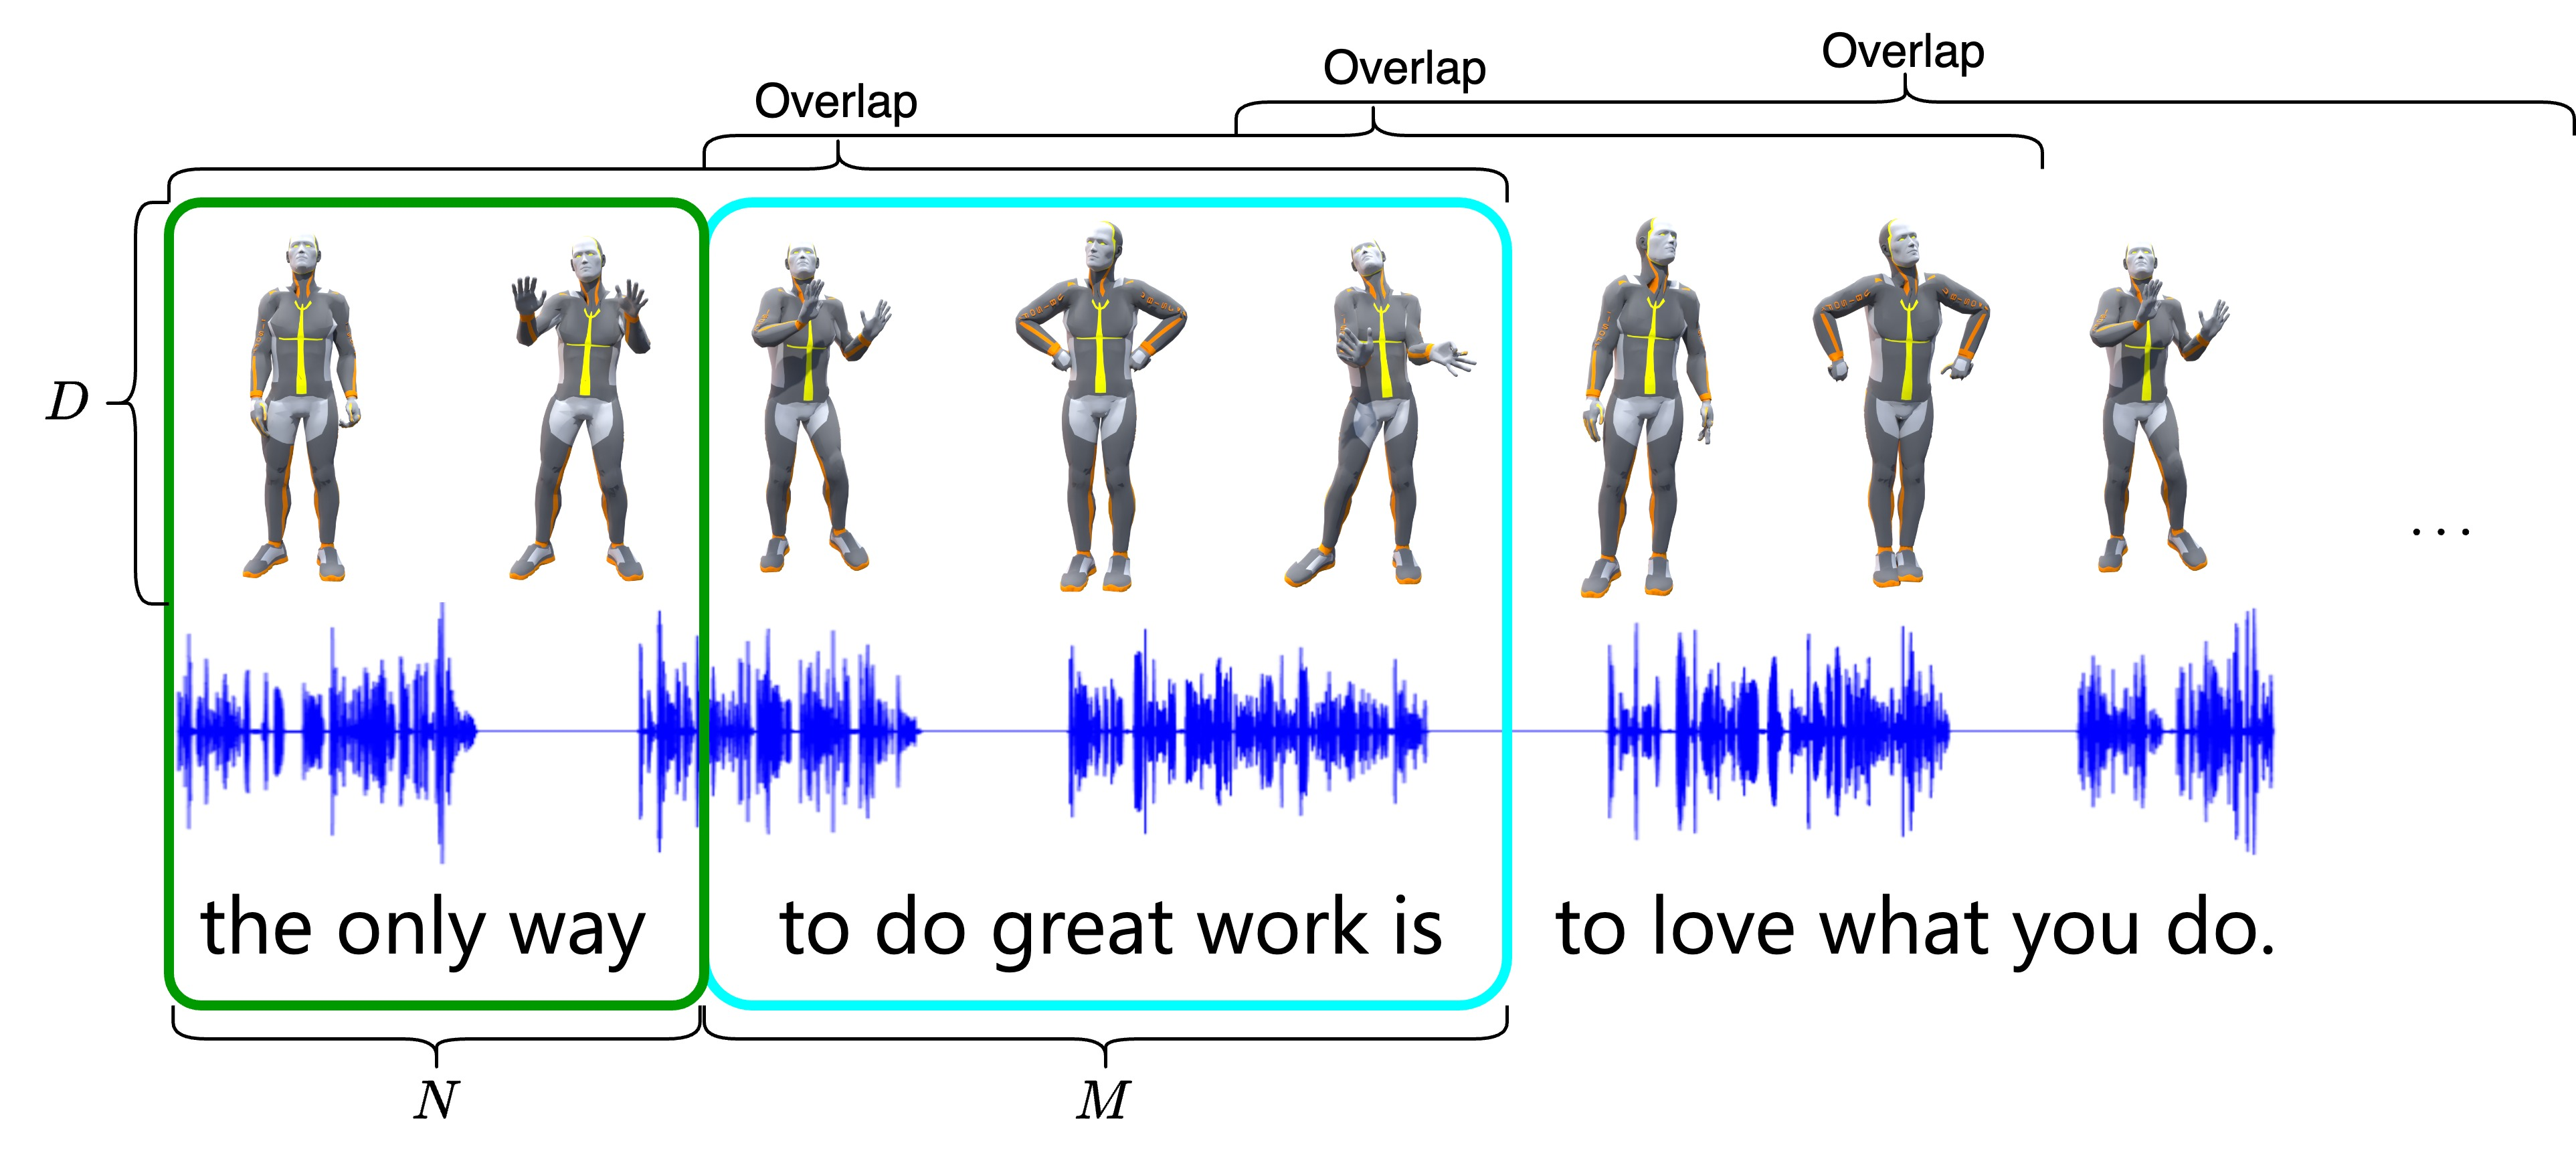
\includegraphics[height=4.5cm]{GestureSeries}
\end{figure}

\vspace{-10pt}

\begin{columns}
	
	\begin{column}{0.6\textwidth}
		
		\textbf{Input}
		\begin{itemize}
			\item Chuỗi cử chỉ khởi tạo: $\mathbf{s} \in \mathbb{R}^{N \times D}$
			\item Chuỗi âm thanh: $\mathbf{a}^{length}$ sample rate 16000 được cắt thành từng đoạn 4s: $\mathbf{a} \in \mathbb{R}^{6400}$
%			trích xuất đặc trưng MFCC: $\mathbf{a} \in \mathbb{R}^{M \times C_{\text{mfcc}}}$
			\item Cảm xúc: $\mathbf{e} \in \mathbb{R}^6$ (\texttt{Happy},  \texttt{Sad},  \texttt{Neutral}, \texttt{Angry}, \texttt{Old}, \texttt{Funny})
			\item Văn bản: $\text{"Love what you do"}$
		\end{itemize}
		
	\end{column}
	\begin{column}{0.4\textwidth}
		 \textbf{Output}
		 \begin{itemize}
		 	\item Chuỗi cử chỉ dự đoán: $\hat{\mathbf{x}} \in \mathbb{R}^{M \times D}$
		 \end{itemize}
		 
		 \textbf{Grouth Truth}
		 \begin{itemize}
		 	\item Chuỗi cử chỉ gốc: $ \mathbf{x}  \in \mathbb{R}^{M \times D}$
		 \end{itemize}
	\end{column}
\end{columns}

\end{frame}

\begin{frame}{Khung chương trình}
	Sử dụng mô hình Diffusion Classifier-Free Guidance (có điều kiện) với cử chỉ $\bx^{1:M \times D}$ làm $x_0$ và điều kiện $c = [{\mathbf{s}, \mathbf{a}, \mathbf{e}}]$. $N = 8$, $M = 80 \sim \text{4 giây}$
	\vspace{-15pt}
%	$N=8$ khung hình đầu làm khởi tạo và $M=80$ khung hình để dự đoán
		\begin{figure}[h]
			\centering
			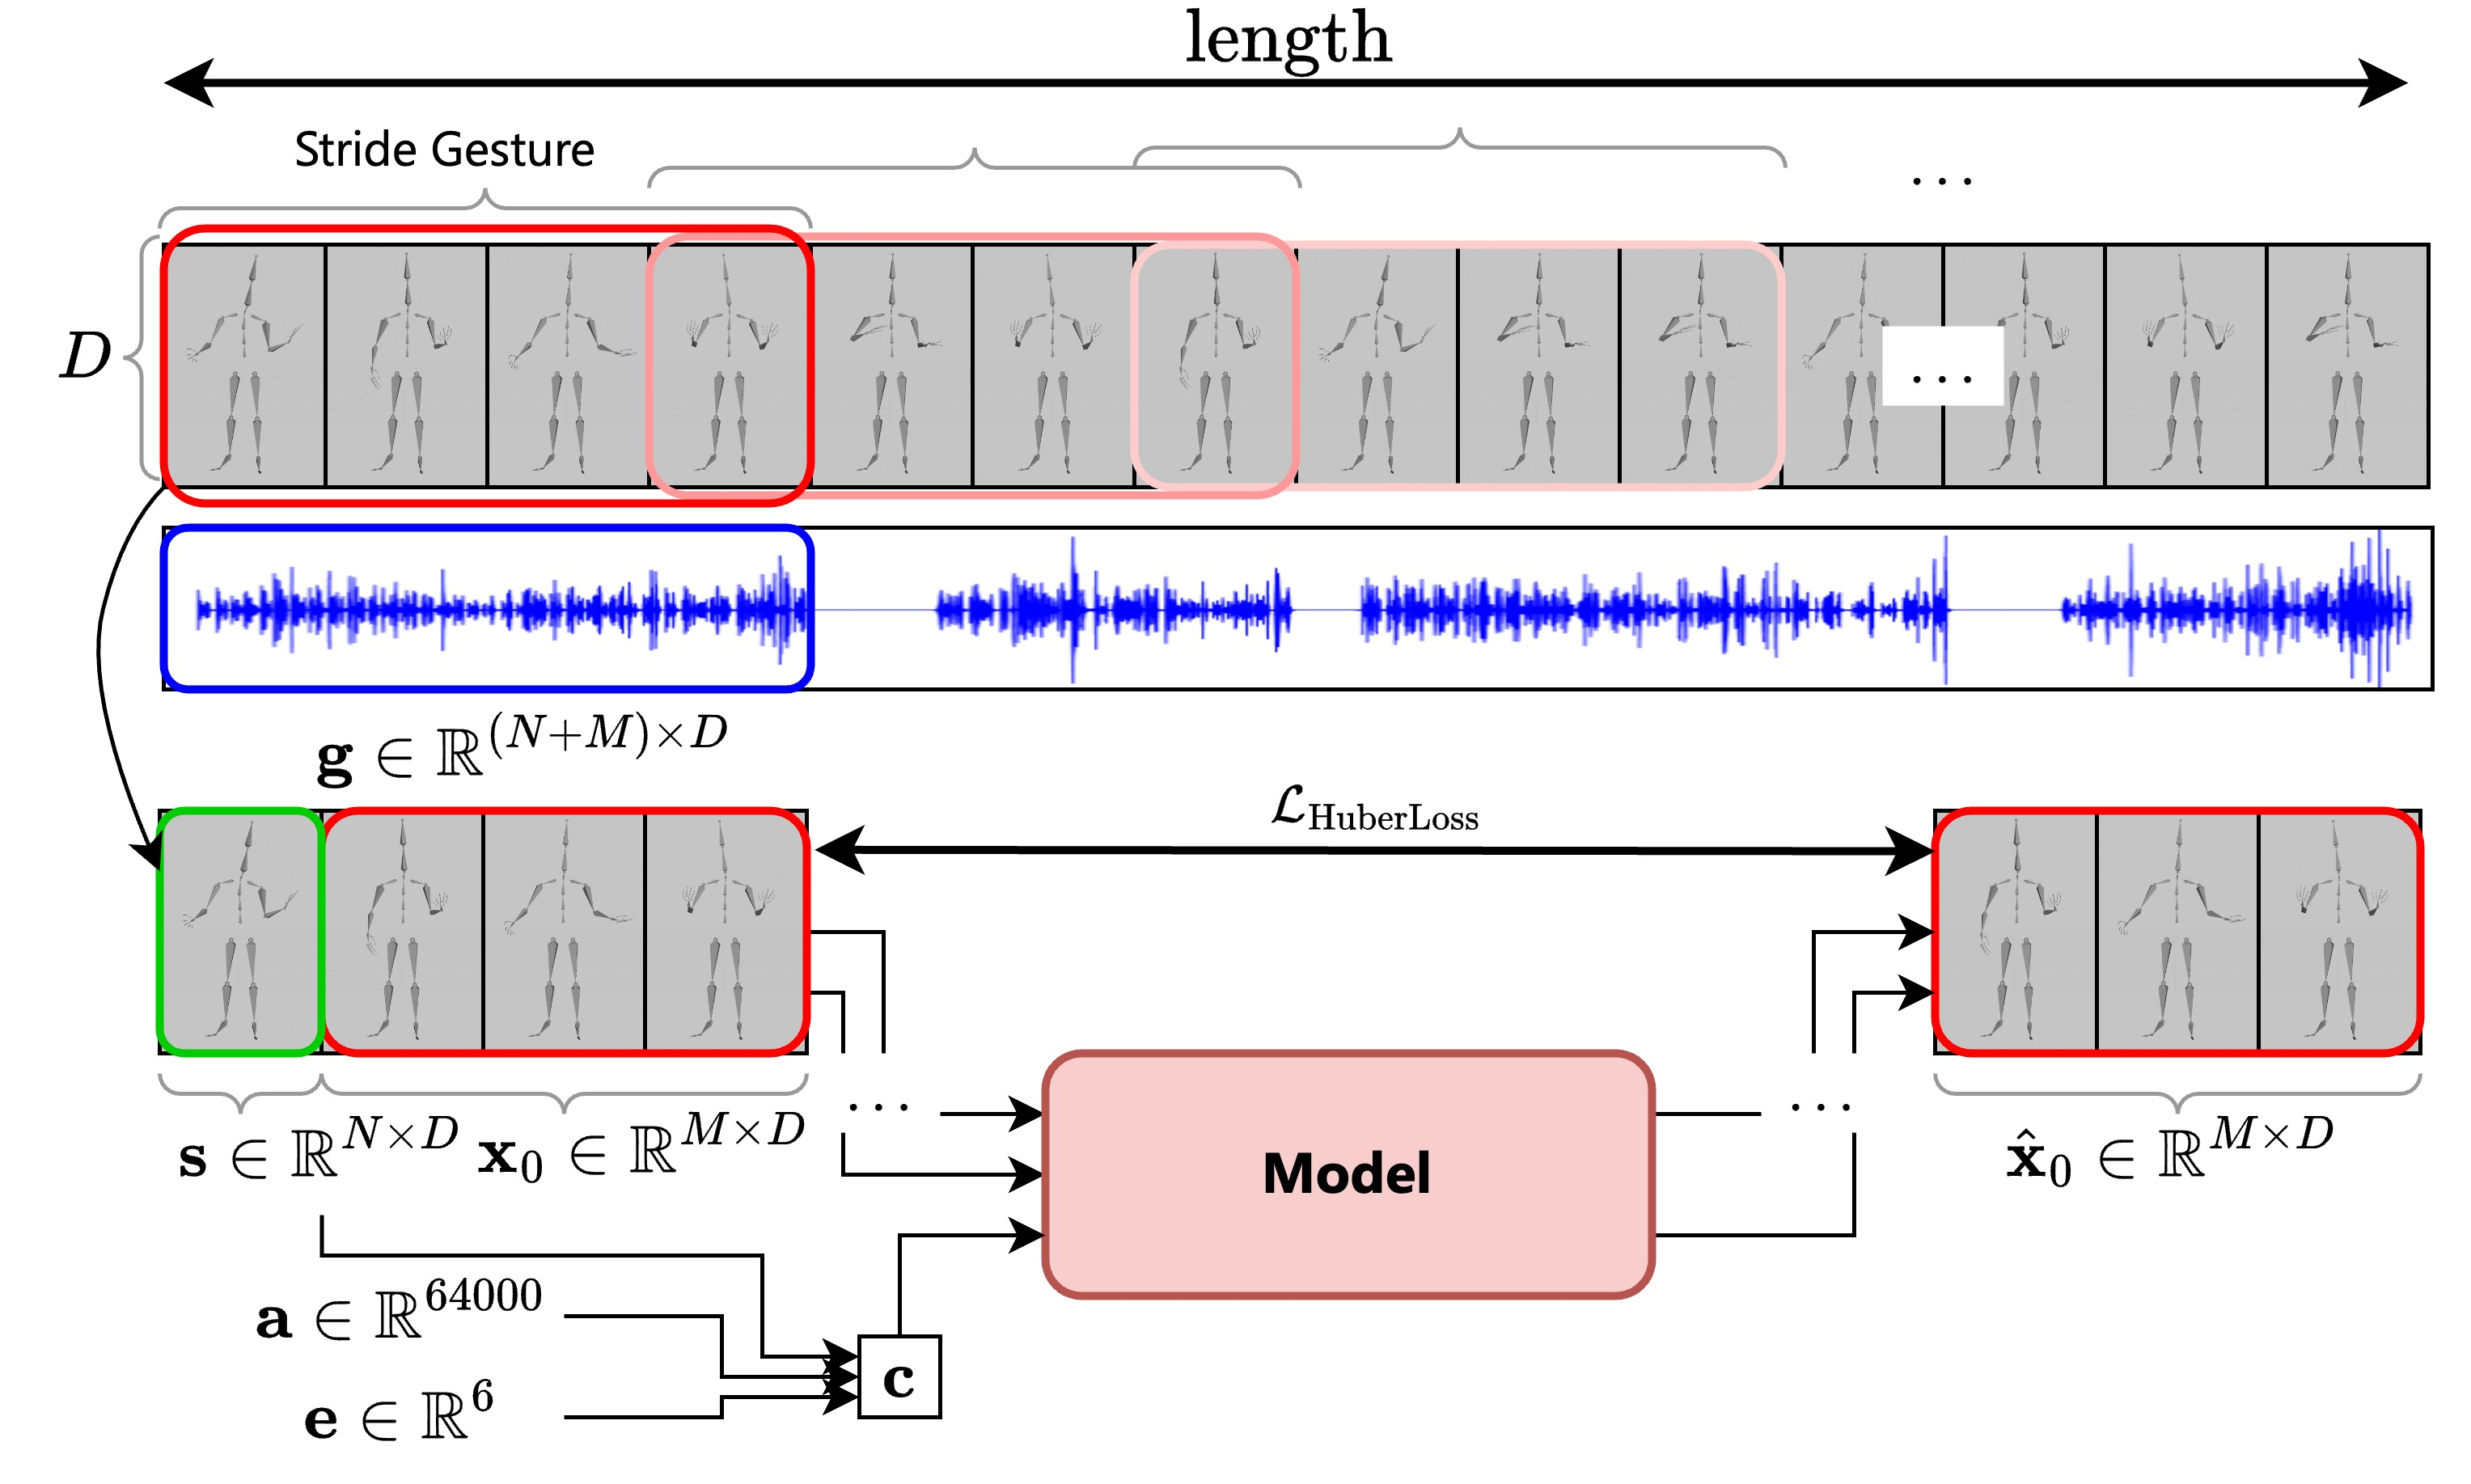
\includegraphics[width=0.95\textwidth]{Framework}
		\end{figure}
	
%\textbf{Training}
%	\begin{itemize}
%		\item $f_{\theta}(\mathbf{g}_0, \mathbf{a}, \mathbf{e})$
%	\end{itemize}
%
%\textbf{Inference}
%
%	\begin{itemize}
%		\item $\mathbf{x}' = f_{\theta'}$
%	\end{itemize}
%Dữ liệu phải được chuẩn hóa trên toàn bộ tập dữ liệu với $\mu(g) = 0$ và $\sigma = 1$. $\bx_{i} = \frac{\bx_{i} - \mu}{\sigma}$.

\end{frame}

%\[
%\begin{array}{ll}
%\mbox{minimize} & f(x) + \lambda \sum_{i=1}^N \|x_i\|_2
%\end{array}
%\]


%\begin{frame}{Structured group lasso \\[-0.3em] 
%{\footnotesize \textmd{(Jacob, Obozinski, Vert; Bach et al.; Zhao, Rocha, Yu; \dots)}}}
%\begin{itemize}\itemsep=12pt
%\item problem:
%\[
%\begin{array}{ll}
%\mbox{minimize} & f(x) + \sum_{i=1}^N \lambda_i \|x_{g_i}\|_2
%\end{array}
%\]
%where $g_i \subseteq [n]$ and $\mathcal G = \{g_1, \dots, g_N\}$
%\item like group lasso, but the groups can overlap arbitrarily
%\item particular choices of groups can impose `structured' sparsity
%\item \eg, topic models, selecting interaction terms for (graphical) models,
%    tree structure of gene networks, fMRI data
%\item generalizes to the \textbf{composite absolute penalties family}:
%\[
%r(x) = \|(\|x_{g_1}\|_{p_1}, \dots, \|x_{g_N}\|_{p_N})\|_{p_0}
%\]
%\end{itemize}
%\end{frame}

%\begin{frame}{Structured group lasso \\[-0.3em] 
%{\footnotesize \textmd{(Jacob, Obozinski, Vert; Bach et al.; Zhao, Rocha, Yu; \dots)}}}
%\textbf{hierarchical selection}:
%\begin{center}
%\begin{tikzpicture}
%[dot/.style={rectangle,draw=black,fill=white,inner sep=5pt,minimum size=5pt}]
%\node[dot,draw=orange,thick] at (0,5) (n1) {1};
%\node[dot] at (-1,4) (n2) {2};
%\node[dot,draw=orange,thick] at (1,4) (n3) {3};
%\node[dot] at (-1,3) (n4) {4};
%\node[dot,draw=orange,thick] at (0.5,3) (n5) {5};
%\node[dot] at (1.5,3) (n6) {6};
%\draw[->] (n1) -- (n2);
%\draw[->] (n1) -- (n3);
%\draw[->] (n2) -- (n4);
%\draw[->] (n3) -- (n5);
%\draw[->] (n3) -- (n6);
%\end{tikzpicture}
%\end{center}
%\begin{itemize}\itemsep=8pt
%    \item $\mathcal G = \{ \{4\}, \textcolor{orange}{\{5\}}, \{6\}, \{2,4\}, 
%        \textcolor{orange}{\{3,5,6\}}, \textcolor{orange}{\{1,2,3,4,5,6\} \}}$
%\item nonzero variables form a rooted and connected subtree
%    \begin{itemize}
%        \item if node is selected, so are its ancestors
%        \item if node is not selected, neither are its descendants
%    \end{itemize}
%\end{itemize}
%\end{frame}

%\begin{frame}[fragile]{Sample ADMM implementation: lasso}
%\begin{verbatim}
%prox_f = @(v,rho) (rho/(1 + rho))*(v - b) + b;
%prox_g = @(v,rho) (max(0, v - 1/rho) - max(0, -v - 1/rho));
%
%AA = A*A';
%L  = chol(eye(m) + AA);
%
%for iter = 1:MAX_ITER
%    xx = prox_g(xz - xt, rho);
%    yx = prox_f(yz - yt, rho);
%
%    yz = L \ (L' \ (A*(xx + xt) + AA*(yx + yt)));
%    xz = xx + xt + A'*(yx + yt - yz);
%  
%    xt = xt + xx - xz;
%    yt = yt + yx - yz;
%end
%\end{verbatim}
%\end{frame}

